\documentclass{article}

\usepackage{ragged2e}
\usepackage{graphicx}
\usepackage{amsmath}
\usepackage{siunitx}

\begin{document}

\begin{flushright}
    \noindent
    Rodrigo Becerril Ferreyra\\
    CECS 211 Section 01\\
    Lab 2\\
    2019-09-05
\end{flushright}

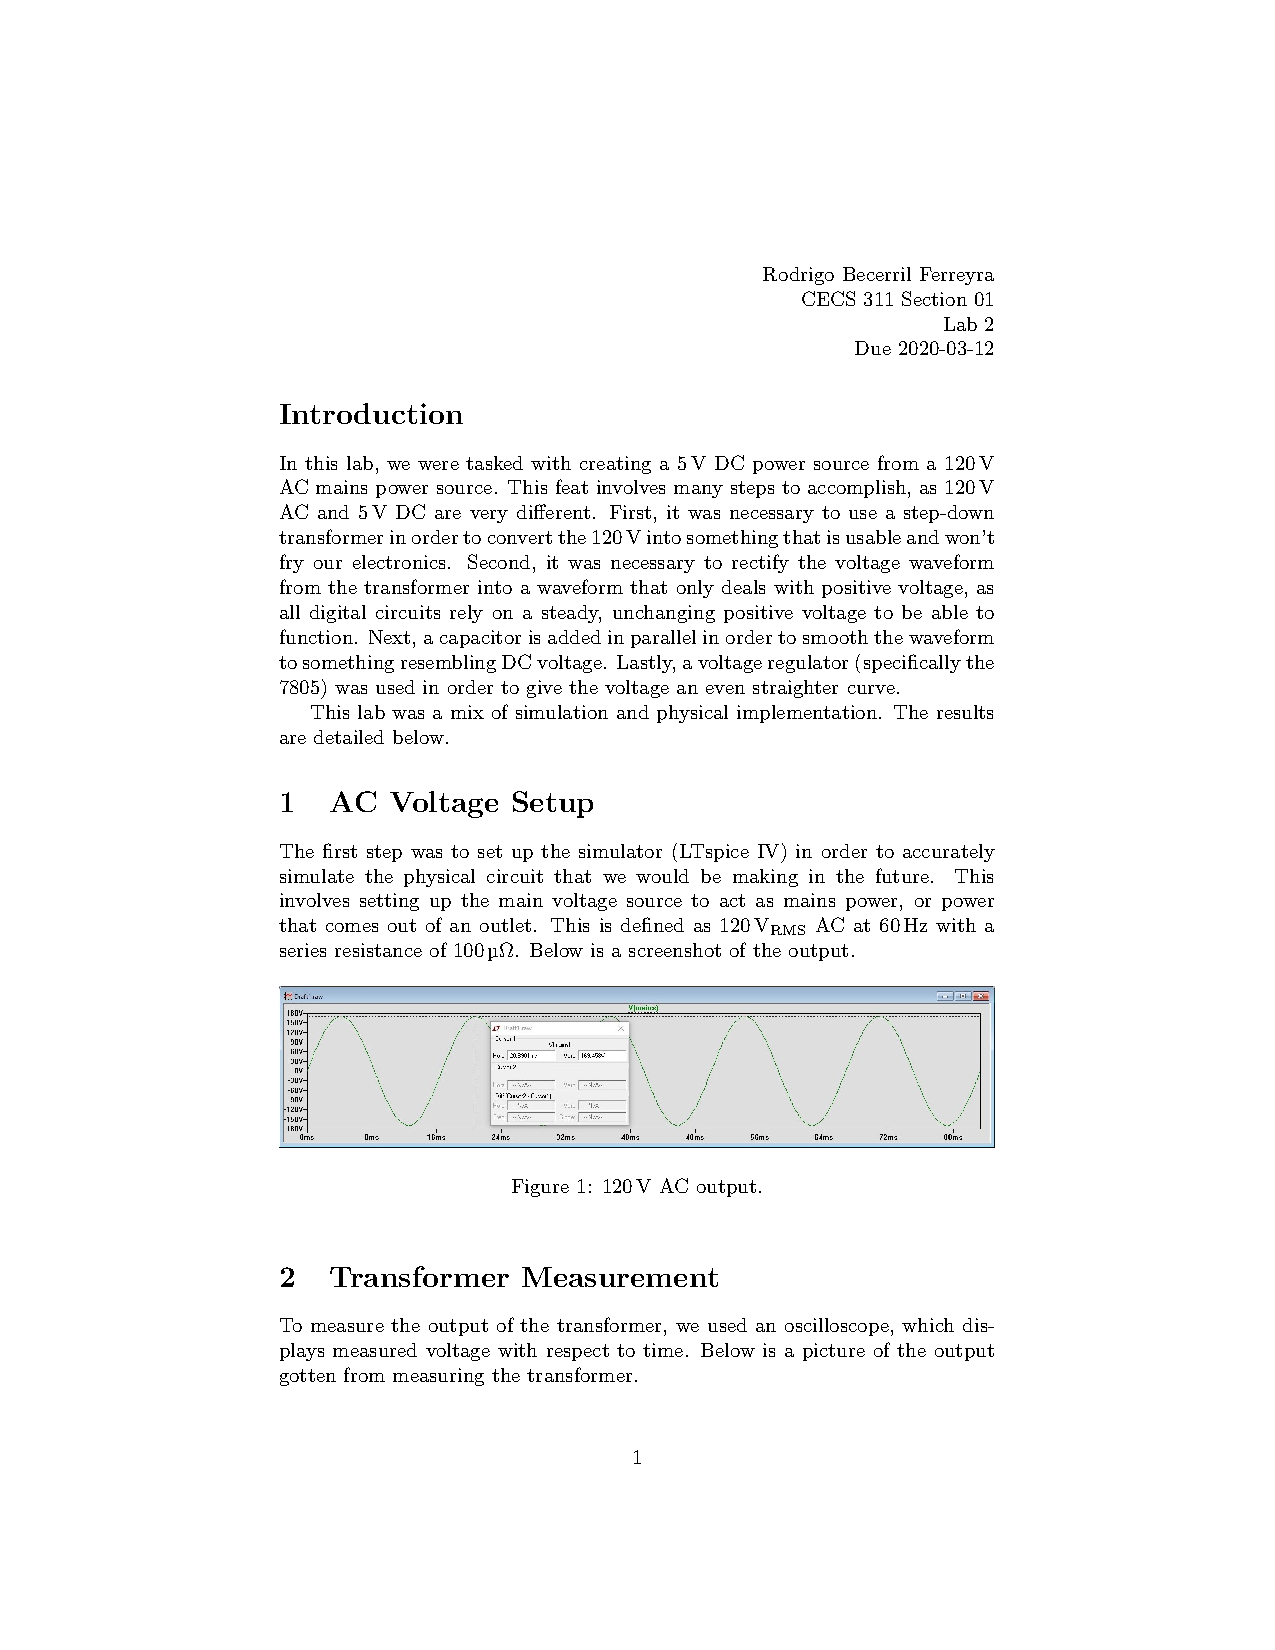
\includegraphics[width=\textwidth]{Lab2.png}

This screenshot shows KVL in action by displaying various
voltage values across three resistors with different values.

\textbf{Total resistance:}
The resistance of $R_1$ is \SI{1}{\kilo\ohm}, the resistance of
$R_2$ is \SI{4.02}{\kilo\ohm}, and the resistance of $R_3$ is
\SI{4.99}{\kilo\ohm}; the total resistance $R_\text{net}$ is
$(1 + 4.02 + 4.99)\ \si{\kilo\ohm} = \SI{10.01}{\kilo\ohm}$.

\textbf{XMM5:}
Ohm's Law $(V=IR)$ can be modified to find the current of
a circuit when the voltage and resistance are known:
$I = V/R$. Plugging in $V$ and $R$ into this equation:

\begin{align*}
    I = \frac{V}{R} = \frac{V_s}{R_\text{net}} &= \frac{\SI{12}{\volt}}{\SI{10.01e3}{\ohm}}\\
    &= \SI{0.001199}{\ampere} = \SI{1.199}{\milli\ampere}
\end{align*}

This value is displayed in XMM5.

\textbf{XMM1, XMM2, and XMM3:}
This is an example of KVL. The amount of
voltage going through each resistor can be calculated by Ohm's
Law: $V=IR$. Plugging in the amount of current $I$
that was calculated in the last
section (\SI{1.199}{\milli\ampere}) and the amount of
resistance of $R_1$ which is \SI{1}{\kilo\ohm}, we can calculate
the following:

\begin{align*}
    V_{R_1} = IR_1 &= (\SI{1.199e-3}{\ampere})(\SI{1e3}{\ohm}) \\
    &= \SI{1.199}{\volt}
\end{align*}

\pagebreak

This is indeed the value displayed by XMM1. Calculating
the expected values for XMM2 and XMM3 can be calculated
in a similar way:

\begin{align*}
    V_{R_2} = IR_2 &= (\SI{1.199e-3}{\ampere})(\SI{4.02e3}{\ohm})\\
    &= \SI{4.82}{\volt}
\end{align*}

\begin{align*}
    V_{R_3}=IR_3 &= (\SI{1.199e-3}{\ampere})(\SI{4.99e3}{\ohm})\\
    &= \SI{5.98}{\volt}
\end{align*}

The XMM2 and XMM3 digital multimeters display the values
\SI{4.819}{\volt} and \SI{5.982}{\volt}, respectively.
These values are the same as were calculated
(to two decimal points). Thanks to KVL, the three values for
voltage across the three resistors add up to the original
voltage of the DC power source:

\begin{gather*}
    \text{Clockwise from the top-left corner, before XMM5:}\\
    +V_{R_1} + V_{R_2} + V_{R_3} - V_s = \SI{0}{\volt}\\
    +\SI{1.199}{\volt} + \SI{4.82}{\volt} + \SI{5.98}{\volt} - \SI{12}{\volt} = \SI{0}{\volt}\\
    \SI{-0.001}{\volt} = \SI{0}{\volt}
\end{gather*}

\noindent (The last line is due to rounding error.)

\textbf{XMM4:}
XMM4 is unique due to the fact that it is spanning two
resistors instead of only one. This means that it is measuring
the voltage going across two resistors. The amount of voltage can be
inferred to be higher than any other singular measurement,
because the resistance is higher, and voltage and resistance
are directly proportional quantities. The expected value
of the measurement can once again be acquired through the use
of Ohm's Law, adding together the resistances of $R_2$ and $R_3$:

%Add variables like $R_1$ before inputting numbers
\begin{align*}
    V_{R_{2+3}} &= I(R_2 + R_3)\\
    &= (\SI{1.199e-3}{\ampere})
    (\SI{4.02e3}{\ohm} + \SI{4.99e3}{\ohm})\\
    &= (\SI{1.199e-3}{\ampere})(\SI{9.01e3}{\ohm})\\
    &= \SI{10.80}{\volt}
\end{align*}

Sure enough, this is the value displayed on XMM4.
An interesting but expected observation that could be made
is the fact that the readings in XMM1 and XMM4 add up to
the total amount of voltage applied to the circuit by the
power source; that is,
$\SI{1.199}{\volt} + \SI{10.801}{\volt} = \SI{12}{\volt}$.
This is another example of KVL in action in a circuit.

\end{document}
